We wczesnych latach 50' XX wieku, firma Toyota stworzyła System produkcyjny Toyoty (ang. \emph{Toyota Production System})
bazujący na wcześniejszych doświadczeniach związanych z usuwaniem marnotrawstwa i ciągłym
udoskonalaniem procesu. System produkcyjny Toyoty jest uważany za prekursora metodyki Lean. Kładł on nacisk na pozbywanie się marnotrawstwa (ang. \textit{removal of waste}), usprawnianie przepływu (ang. \textit{improving flow}) oraz 
poprawianie ogólnej oceny produktu z puntu widzenia klienta (ang. \emph{customer value}).

Six Sigma zrodziła się w firmie Motorola w latach 80' XX wieku. Stworzył ją 
dyrektor generalny Motoroli w trakcie realizacji wyzwania polegającego na dziesięciokrotnym udoskonaleniu jakości produktów w ciągu pięciu lat.
W trakcie, gdy kierownicy Motoroli szukali sposobu, żeby uzyskać ten cel, inżynier
Bill Smith analizował korelację pomiędzy czasem życia produktu, a tym jak często 
produkt był naprawiany w trakcie produkcji.
\begin{figure}[!htp]
	\centering
	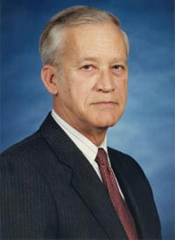
\includegraphics[width=0.25\textwidth]{img/bill-smith2}
	\caption{Bill Smith znany jako ,,Ojciec metodologii Six Sigma''}
\end{figure}
Wykazał, że jeżeli produkt
został uznany za uszkodzony i został naprawiony w czasie produkcji, inne
usterki zostawały przeoczone i ujawniały się we wczesnym okresie użytkowania przez klienta. Jeżeli natomiast produkt został uznany za sprawny, rzadko pojawiały się 
w nim wady u klienta. Doprowadziło to do narodzin metodologii Six Sigma.
Początkowo Six Sigma było zwyczajną metryką, miarą jakości procesu.
Six Sigma to pogoń za jakością określającą nie więcej niż 3,4 usterek na milion sposobności
(ang. 3.4\emph{DPMO}, \emph{Defects Per Milion Opportunities}).

Do roku 1993 Motorola osiągnęła poziom jakości Six Sigma w każdym zakładzie produkcyjnym.
Pozostałe firmy zaczęły brać udział w rewolucji jakościowej ---
Honeywell (później Allied Signal), Texas Instruments, Eastman Kodak jako pierwsze
zaadoptowały metodykę Six Sigma u siebie we wczesnych latach 90' XX wieku.
Stworzono metodę MAIC (ang. \textit{Measure, Analyze, Improve and Control}) służącą
do  wdrażania metodologii Six Sigma do istniejącego procesu.

W 1995 roku, General Electrics zaczął korzystać z Six Sigma. Dyrektor generalny
GE Jack Welch stał się jednym z największych obrońców tej metodyki.
\begin{figure}[!htp]
	\centering
	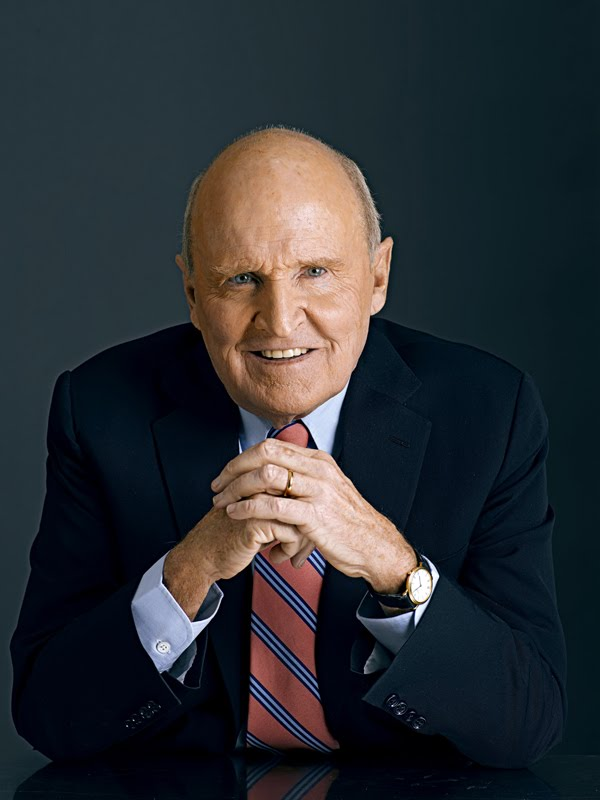
\includegraphics[width=0.25\textwidth]{img/welch}
	\caption{Dyrektor generalny General Electrics --- Jack Welch}
\end{figure}
GE wprowadziło również fazę \emph{Define} jako pierwszą fazę do metody MAIC (tak powstao \textit{DMAIC}). Do roku 
2001, firma GE odnotowała oszczędność 4,5 biliona dolarów jako bezpośredni
rezultat działania Six Sigma.

Ostatecznie, na początku pierwszej dekady XXI w., wiele firm zaczęło łączyć metodyki Lean oraz Six Sigma we wszechstronną metodologię usprawnieniową znana obecnie jako Lean Six Sigma.